\documentclass{article}



\usepackage{IEEEtrantools}
\usepackage{amsmath}
\usepackage{mathrsfs}
\usepackage{graphicx}
\usepackage{subcaption}
\usepackage{setspace}
\usepackage{color}
\usepackage[margin=0.7in]{geometry}

\newcommand{\C}{\mathbf{C}}
\newcommand{\h}{\mathbf{h}}
\renewcommand{\r}{\mathbf{r}}
\newcommand{\x}{\mathbf{x}}
\newcommand{\A}{\mathbf{A}}
\newcommand{\Z}{\mathbf{Z}}
\newcommand{\Y}{\mathbf{Y}}
\newcommand{\X}{\mathbf{X}}
\newcommand{\N}{\mathcal{N}}
\newcommand{\w}{\mathbf{w}}
\newcommand{\logit}{\text{logit}}


\begin{document}

  \section{Context}

  \paragraph{Objectives:}

  Here I want to predict the nutrient flux because it can give us an idea about new production. This amount of new production is difficult to estimate without data at high temporal resolution with existing methods [aqaba paper]. Therefore if there is a method that allows us to do that just using satellite data that would be great.

  \paragraph{Data:}

  I clustered the red sea into 8 provinces bases on monthly chl patterns. [cluster figure] I want interested in the cluster nb ? during winter 1999-2000 because there is an important bloom in this region. I averaged daily SeaWifs data from [] to [] in the given cluster, giving me the following time series [figure], that is to say [] nb of measurements.  


  \begin{figure}[ht]
  \centering
    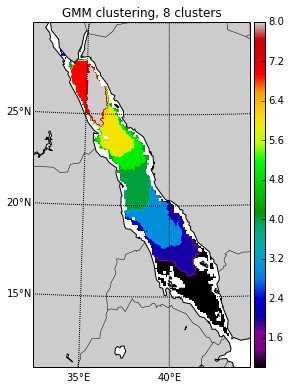
\includegraphics[scale=.3]{./clusters.png}
  \caption{Result of clustering. We are interested in the red region.}
  \end{figure}


  \begin{figure}[ht]
  \centering
    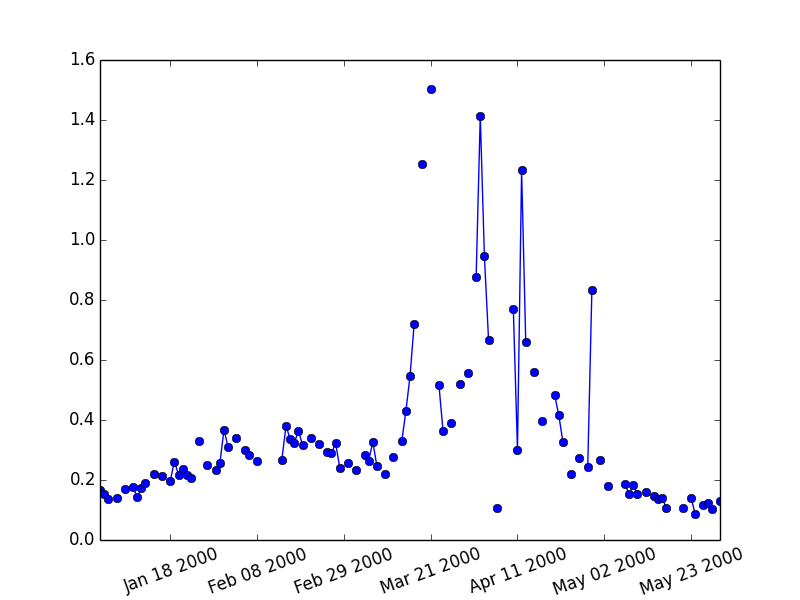
\includegraphics[scale=.3]{./chl_ts.png}
  \caption{Averaged of CHL concentration in studied cluster: The data to be used in the inversion.}
  \end{figure}


  \paragraph{Box model:}

  We assume that a box model or 0d model represents the mixed layer in the cluster region we are interested in, and futhermore that there is no exchange with the neighboring regions and that the input of nutrient just come from the deep sea. We only model the phytoplankton, the nutrient concentration (we assume that the nitrate is the limiting nutrient), and the grazing pressure through a zooplankton concentration. A certain part of the zooplankton and phytoplankton is assumed to be lost by sinking, whereas a stochastic term models a flux of nutrient that diffuse to the mixed layer from the deep water. This is that term that we are interested in estimating.

  \paragraph{NPZ model:}

  The NPZ model is the simplest meaningful model for the phytoplankton
  growth. It is a ODE model that links phytoplankton concentrations 
  (\textcolor{green}{P}) to preying zooplankton (\textcolor{red}{Z}) and
  available nutrient (\textcolor{blue}{N}) concentrations. In our case we 
  augment the NPZ model by including a nutrient flux term ($\Phi$) that 
  models an input of nutrient from the deep sea. The equations of the
  NPZ model are shown below:

  \begin{IEEEeqnarray}{rCl}
    \textcolor{green}{\frac{dP}{dt}} & = & 
    \textcolor{green}{\mu\frac{N}{k+N}P} 
    - \textcolor{red}{gPZ} 
    - \textcolor{green}{\varepsilon_PP}
    - \textcolor{green}{\varepsilon_P^* P^2},\\
    \textcolor{red}{\frac{dZ}{dt}} & = & 
    \textcolor{red}{\gamma gPZ} 
    - \textcolor{red}{\varepsilon_ZZ}
    - \textcolor{red}{\varepsilon_Z^*Z^2},\\
    \textcolor{blue}{\frac{dN}{dt}} & = &
    -\textcolor{green}{\mu\frac{N}{k+N}P} 
    + \textcolor{red}{(1-\gamma)gPZ} 
    + \textcolor{green}{\varepsilon_PP} 
    + \textcolor{red}{\varepsilon_ZZ} 
    + \Phi_N(t).
  \end{IEEEeqnarray}


  \section{Statistical modeling}

  Denote $Y_1, ..., Y_T$ the observations of chlorophyll
  concentration, $\X_1, ..., \X_T$ the state variables, with
  $\X_t = \left[N_t, P_t, Z_t, \Phi_t\right]^T$, the concentration of each of the
  ODE state variables at time $t$. For now on, we actually considere the log
  of these concentrations. 

  \begin{figure}[ht]
  \centering
    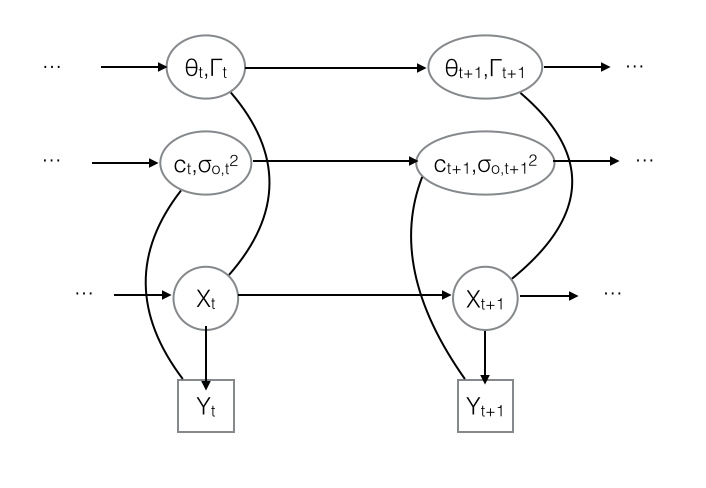
\includegraphics[scale=.3]{./BHM3.jpg}
  \caption{BHM second attempt}
  \end{figure}

  \subparagraph{Data model:}

  The observations are independent conditionally on the state of the system.

  \begin{IEEEeqnarray}{c}
  	Y_t = c_t + P_t + w^o_t,
  \end{IEEEeqnarray}

  with $w^o_t \sim \N(0, (\sigma^o_t)^2)$ iid and $c_t$ in the log-conversion
  rate between the chlorophyll and the phytoplankton concentrations. 


  \subparagraph{Process model:}

  The state variables are assumed Markovian:

  \begin{IEEEeqnarray}{c}
    X_t = \left[
      \begin{array}{c}
        N_t \\P_t\\ Z_t \\ \Phi_t
      \end{array}\right] = 
    \left[\begin{array}{c} f(X_{t-1};\theta_t)\\ \Phi_{t-1}
      \end{array}\right] + \w_t, \w_t \sim \N(0, diag(\Gamma_t))
  \end{IEEEeqnarray}

	$f$ is the result of the integration of the ODE system between times 
	$t-1$ and $t$ with initial conditions $\left[N_{t-1}, P_{t-1}, Z_{t-1}
	\right]$ and a fixed nutrient flux $\Phi_{t-1}$. 
  $\Gamma_t = \left[(\sigma_t^N)^2, 
  (\sigma_t^P)^2, (\sigma_t^Z)^2, (\sigma_t^\Phi)^2\right]$.
  $\Phi_t$ is a random walk process. 


  \subparagraph{Transition model:}

  We denote: $\lambda_t = [\theta^T_t, \Gamma^T_t, c_t, \sigma^o_t]^T$

  We have to specify a transition model for the time-varying parameters. We choose a random walk process of the form:

  \begin{IEEEeqnarray}{c}
    \logit (\lambda^{(i)}_{t+1}) = \logit (\lambda^{(i)}_t) + v^{(i)}_t,
    \text{ if } \lambda^{(i)}_t = \gamma_t, \\
    \log (\lambda^{(i)}_{t+1}) = \log (\lambda^{(i)}_t) + v^{(i)}_t,
    \text{ otherwise},
  \end{IEEEeqnarray}

 where $v^\lambda_t$ is a iid Gaussian random error of fix variance.  



\section{EM methodology}



\section{Case where $\theta$ is known}


\section{Case where $\theta$ is unknown}




\end{document}

